%% Basierend auf einer TeXnicCenter-Vorlage von Tino Weinkauf.
%%%%%%%%%%%%%%%%%%%%%%%%%%%%%%%%%%%%%%%%%%%%%%%%%%%%%%%%%%%%%%

%%%%%%%%%%%%%%%%%%%%%%%%%%%%%%%%%%%%%%%%%%%%%%%%%%%%%%%%%%%%%
%% HEADER
%%%%%%%%%%%%%%%%%%%%%%%%%%%%%%%%%%%%%%%%%%%%%%%%%%%%%%%%%%%%%
\documentclass[a4paper,oneside,12pt]{article}
\usepackage{geometry}
\geometry{a4paper,left=40mm,right=30mm, top=25mm, bottom=25mm} 
% Alternative Optionen:
%	Papiergr��e: a4paper / a5paper / b5paper / letterpaper / legalpaper / executivepaper
% Duplex: oneside / twoside
% Grundlegende Fontgr��en: 10pt / 11pt / 12pt


%% Deutsche Anpassungen %%%%%%%%%%%%%%%%%%%%%%%%%%%%%%%%%%%%%
\usepackage[ngerman]{babel}
\usepackage[utf8]{inputenc}
\usepackage[T1]{fontenc}
\usepackage{lmodern} %Type1-Schriftart f�r nicht-englische Texte
\usepackage{float}
\usepackage{floatflt}

%% Packages f�r Grafiken & Abbildungen %%%%%%%%%%%%%%%%%%%%%%
\usepackage{graphicx} %%Zum Laden von Grafiken
%\usepackage{subfig} %%Teilabbildungen in einer Abbildung
%\usepackage{pst-all} %%PSTricks - nicht verwendbar mit pdfLaTeX

%% Beachten Sie:
%% Die Einbindung einer Grafik erfolgt mit \includegraphics{Dateiname}
%% bzw. �ber den Dialog im Einf�gen-Men�.
%% 
%% Im Modus "LaTeX => PDF" k�nnen Sie u.a. folgende Grafikformate verwenden:
%%   .jpg  .png  .pdf  .mps
%% 
%% In den Modi "LaTeX => DVI", "LaTeX => PS" und "LaTeX => PS => PDF"
%% k�nnen Sie u.a. folgende Grafikformate verwenden:
%%   .eps  .ps  .bmp  .pict  .pntg


%% Packages f�r Formeln %%%%%%%%%%%%%%%%%%%%%%%%%%%%%%%%%%%%%
\usepackage{amsmath}
\usepackage{amsthm}
\usepackage{amsfonts}


%% Zeilenabstand %%%%%%%%%%%%%%%%%%%%%%%%%%%%%%%%%%%%%%%%%%%%
%\usepackage{setspace}
%\singlespacing        %% 1-zeilig (Standard)
%\onehalfspacing       %% 1,5-zeilig
%\doublespacing        %% 2-zeilig


%% Farben %%%%%%%%%%%%%%%%%%%%%%%%%%%%%%%%%%%%%%%%%%%%%%%%%%%
\usepackage{color}
\usepackage{framed}
\usepackage{colortbl}
\definecolor{middlegray}{rgb}{0.5,0.5,0.5}
\definecolor{lightgray}{rgb}{0.8,0.8,0.8}
\definecolor{orange}{rgb}{0.8,0.3,0.3}
\definecolor{yac}{rgb}{0.6,0.6,0.1}
\definecolor{darkgray}{rgb}{0.3,0.3,0.3}
\definecolor{blue}{rgb}{0,0,1}
\definecolor{green}{rgb}{0,0.6,0}
\definecolor{yellow}{rgb}{1,1,0}
\definecolor{shadecolor}{gray}{.85}
\usepackage[table]{xcolor}
\newcommand{\tblue}{\cellcolor{blue!25}}
\newcommand{\tred}{\cellcolor{red!25}}
\newcommand{\tgreen}{\cellcolor{green!25}}
\newcommand{\tyellow}{\cellcolor{yellow!25}}


%% CodeListings %%%%%%%%%%%%%%%%%%%%%%%%%%%%%%%%%%%%%%%%%%%%%
\usepackage{listings}
\lstset{
	basicstyle=\scriptsize\ttfamily,
	keywordstyle=\bfseries\ttfamily\color{blue},
	breaklines=true,
	stringstyle=\color{darkgray}\ttfamily,
	commentstyle=\color{green}\ttfamily,
	emph={square}, 
	emphstyle=\color{blue}\texttt,
	emph={[2]root,base},
	emphstyle={[2]\color{yac}\texttt},
	showstringspaces=false,
	flexiblecolumns=false,
	captionpos=b,
	tabsize=2,
	numbers=left,
	numberstyle=\tiny,
	numberblanklines=true,
	stepnumber=1,
	numbersep=10pt,
	xleftmargin=15pt,
	frame=single
}

%% Verlinktes Inhaltsverzeichnis %%%%%%%%%%%%%%%%%%%%%%%%%%%
\usepackage[colorlinks,
pdfpagelabels,
pdfstartview = FitH,
bookmarksopen = true,
bookmarksnumbered = true,
linkcolor = black,
plainpages = false,
hypertexnames = false,
citecolor = black] {hyperref}


%% Sonstiges %%%%%%%%%%%%%%%%%%%%%%%%%%%%%%%%%%%%%%%%%%%%%%%
\usepackage{float}
\usepackage{tabularx}
\usepackage{amsmath}
\usepackage{subfigure}
\usepackage{multirow}
\usepackage{ulem}
\usepackage{wrapfig}

\setlength{\parindent}{0pt}


%% Andere Packages %%%%%%%%%%%%%%%%%%%%%%%%%%%%%%%%%%%%%%%%%%
%\usepackage{a4wide} %%Kleinere Seitenr�nder = mehr Text pro Zeile.
%\usepackage{fancyhdr} %%Fancy Kopf- und Fu�zeilen
%\usepackage{longtable} %%F�r Tabellen, die eine Seite �berschreiten


%% execute scripts %%%%%%%%%%%%%%%%%%%%%%%%%%%%%%%%%%%%%%%%%%
\newcommand{\visioToPDF}[1] {
	\immediate\write18{convert_scripts\string\\visioToPDF.bat #1}
}


%%%%%%%%%%%%%%%%%%%%%%%%%%%%%%%%%%%%%%%%%%%%%%%%%%%%%%%%%%%%%
%% Anmerkungen
%%%%%%%%%%%%%%%%%%%%%%%%%%%%%%%%%%%%%%%%%%%%%%%%%%%%%%%%%%%%%
%
% Zu erledigen:
% 1. Passen Sie die Packages und deren Optionen an (siehe oben).
% 2. Wenn Sie wollen, erstellen Sie eine BibTeX-Datei
%    (z.B. 'literatur.bib').
% 3. Happy TeXing!
%
%%%%%%%%%%%%%%%%%%%%%%%%%%%%%%%%%%%%%%%%%%%%%%%%%%%%%%%%%%%%%


%%%%%%%%%%%%%%%%%%%%%%%%%%%%%%%%%%%%%%%%%%%%%%%%%%%%%%%%%%%%%
%% Optionen / Modifikationen
%%%%%%%%%%%%%%%%%%%%%%%%%%%%%%%%%%%%%%%%%%%%%%%%%%%%%%%%%%%%%

%\input{optionen} %Eine Datei 'optionen.tex' wird hierf�r ben�tigt.
%% ==> TeXnicCenter liefert m�gliche Optionendateien
%% ==> im Vorlagenarchiv mit (Datei | Neu von Vorlage...).


%%%%%%%%%%%%%%%%%%%%%%%%%%%%%%%%%%%%%%%%%%%%%%%%%%%%%%%%%%%%%
%% DOKUMENT
%%%%%%%%%%%%%%%%%%%%%%%%%%%%%%%%%%%%%%%%%%%%%%%%%%%%%%%%%%%%%
\begin{document}
\thispagestyle{empty}

\title {
	\huge \textsc{HeartRate2Go}
}
	
\author {
	\begin{tabular}{rl}
		\large Matthias Böffel & \small Matrikel Nr.: 864483 \\ 
		\large Patrick Mathias & \small Matrikel Nr.: 864089 \\ 
		\large Markus Nebel & \small Matrikel Nr.: 864681 \\ 
		\large Janina Sauer & \small Matrikel Nr.: 865235 \\ 
	\end{tabular}
}

\maketitle
\vfill
\begin{figure}[H]
\centering
\small Hochschule Kaiserslautern\\University of Applied Sciences\\
\bigskip
\large Betreuer: Prof. Dr.-Ing. Jan Conrad\\
\bigskip

\includegraphics[scale=0.4]{images/hskllogo.jpg}  
\end{figure}

\newpage
\tableofcontents
%\cleardoublepage %Das erste Kapitel soll auf einer ungeraden Seite beginnen.
%\pagestyle{plain} %%Ab hier die Kopf-/Fusszeilen: headings / fancy / ...

%TODOs: 
%
%In der Abgabe sollen die folgenden Elemente enthalten sein:
%1. Kommentierte Quelltexte und alle Dateien, die für das Bauen und Ausführen der Anwendung 		benötigt werden
%2. Eine ausführbare Version Ihrer Anwendung mit einer Beschreibung z.B. als liesmich.txt die darlegt, wie die Anwendung installiert und ausgeführt wird.
%3. Eine Dokumentation des Projekts im PDF-Format, nähere Infos hierzu finden Sie weiter unten
%
%
%
%Die Dokumentation soll mindestens die folgenden Punkte behandeln:
%1. Beschreibung der von Ihnen implementierten Anwendungen und ihrer Funktionalitäten auf Basis des Konzeptpapiers
%2. Welches Framework haben Sie verwendet? Begründen Sie Ihre Auswahl (macht Patrick)
%3. Beschreibung des Software-Designs
%4. Beschreibung des von Ihnen erstellten User Interface
%5. Eine kurze Beschreibung der Bedienung Ihrer Anwendung
%6. Weitere Angaben zu Ihrem Projekt, falls Sie dies für sinnvoll halten
%7. Verwendete Literatur und Quellen
%8. Retrospektive: Kritischer Rückblick und Vergleich der ursprüngliche Planung mit den
%erzielten Ergebnissen (macht Patrick)
%10. Die von allen Projektmitgliedern unterschriebene „Ausgabe der Projektarbeit und
%Nutzungsvereinbarung“ und „Ehrenwörtliche Erklärung“. Die zwei zu verwendenden
%Vordrucke befinden sich am Ende dieses Dokumentes. (Bös Unterschrift fehlt noch)


\newpage
\section{Einleitung} \label{sec:Einleitung}
\subsection{Vorstellung des Projektes} \label{sec:Vorstellung des Projektes}
Im Projekt \textit{HeartRate2Go} geht es darum, mit einer App für eine Android Uhr die Herzfrequenz per Pulsoxymetrie zu messen und diese Messwerte in einer passenden GUI darzustellen. \\
Somit soll der Anwender bei der Kontrolle seines Pulses unterstützt werden und ihm einen guten, verständlichen Überblick bieten. Dies gilt sowohl für eine Ruhemessung, als auch für eine Messung während einer Aktivität. \\
\\
%Ablauf einer Messung, vllt mit Diagramm 
%Anwender trägt Uhr, startet App, wählt Messart aus, Messung startet, evtl Messung beenden, Abfrage über Stimmung, Smartphone zeigt Durchschnittswert an, Smartphone empfängt Daten automatisch von der Uhr, Smartphone zeigt Werte im Balkendiagramm an, GUI öffnen, GUI empfängt Messdaten per tcp über Smartphone (wird vom Smartphone gesteuert), Messdaten werden in GUI eingefügt und graphisch dargestellt, Messwerte können mit vergangen Messungen verglichen und auch gedruckt werden.
\textbf{Ablauf}\\
\\
Für die Nutzung für \textit{HeartRate2Go} sind drei Komponenten nötig:\\
\begin{itemize}
	\item Android-Uhr
	\item Android-Smartphone und
	\item Computer
\end{itemize}

Der Nutzer trägt die Android-Uhr am Handgelenk und startet auf dieser die \textit{HeartRate2Go-App}. Hier wird nun abgefragt, ob er eine Ruhemessung oder eine Aktivitätsmessung durchführen möchte. Anschließend wird die ausgewählte Messung durchgeführt. Bei einer Ruhemessung wird die Messung automatisch beendet, bei der Aktivitätsmessung muss der Benutzer die Messung manuell beenden. 
Nun wird der Anwender nach seiner Stimmung während der Pulsmessung gefragt, hier hat er die Auswahl zwischen gut, ok und schlecht. Außerdem wird der Durchschnittswert der soeben durchgeführten Messung gezeigt.\\
Die Übertragung der Messwerte von der Android-Uhr an das Android-Smartphone verläuft automatisch per Bluetooth. Auf der Smartphone-App werden die Messungen in einem Balkendiagramm angezeigt und bieten so einen ersten Überblick. \\
\\
\begin{figure} [H]
	\centering
		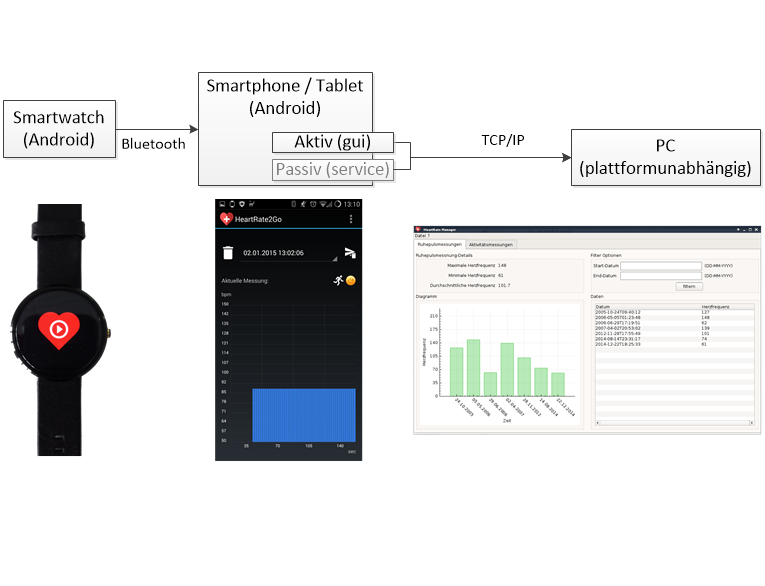
\includegraphics[scale=0.5]{images/ablauf.png}
		\caption{Ablaufdiagramm}
	\label{fig:ablauf}
\end{figure}

\subsection{Medizinische Apps}\label{sec:Medizinische Apps}
Im Laufe der letzten Jahre wurde der Markt mit Apps, die einen medizinischen Hintergrund besitzen, überschüttet. Wenn man im deutschen iTunes-Store nach „Medizin“ sucht, erhält man mehrere hundert Einträge, dies gilt genauso für den Google-Play Store. \\
Im vergangen Jahr sind die Absatzzahlen von medizinischen Apps in Großbritannien, Frankreich, Niederlande und Deutschland um 42 Prozent gestiegen, vermeldet das GfK (Marktforschungszentrum).\\
Diese Apps decken nahezu jeden Bereich der Medizin ab, egal ob es um die Speicherung von Vitaldaten, die Messung von Vitaldaten mit einem zusätzlichen Messgerät und die Auswertung der Daten geht. Des Weiteren sind auch viele Nachschlagewerke darunter enthalten.\\
Zu beachten ist allerdings, dass keiner der Apps den Arztbesuch ersetzt. Sie geben lediglich eine erste Einschätzung und sind dadurch eine große Erleichterung für den Nutzer. Allerdings ist es auch so, dass jeder Programmierer eine App mit medizinischem Hintergrund in die verschiedenen Stores hochladen darf. Diese werde nicht auf ihren Nutzen hin überprüft, so sind auch viele Apps zu finden, die mehr als Spielerei gelten.\\
Kaum eine App ist ein Medizinprodukt nach dem Medizinproduktegesetzt, sie gelten lediglich als Wellness- beziehungsweise Lifestyle-Apps. \\
\\

\textbf{} 
%Thema und Zielsetzung: Stellen Sie zunächst Thema und Zielstellung der Arbeit vor.
%Theorie: Vermitteln Sie Ihre Theorie(n) über das Thema und geben Sie an, auf was sich Ihre Theorie stützt.
%Fragestellung: Teilen Sie mit, welche Fragen in der folgenden Arbeit beantwortet werden.
%Quellen: Welche Quellen haben Sie für Ihre Arbeit genutzt bzw. wie haben Sie Ihre Frage(n) beantwortet?
%Ergebnis: Führen Sie Ihre Ergebnisse auf, also teilen Sie mit, was Sie herausgefunden haben.
%Fazit: Stellen Sie am Ende des Abstracts eine Quintessenz auf. Sie können Ihr Fazit auch mit einer %Zukunftsprognose verbinden.

\subsection{Medizinische Kenntnisse - Pulsoxymetrie} 
Für die Messung des peripheren Pulses per Android-Uhr wird das Prinzip der Reflexions-Pulsoxymetrie genutzt (Abbildung \ref{pic:pulsoxy}).\\
Dieses Verfahren benötigt zwei Sensoren: zum einen eine Lichtquelle, zum anderen ein Lichtsensor. Die Lichtquelle sendet Infrarot-Lichtwellen aus, die durch die Haut dringen. Der Sensor misst die Lichtanteile, die absorbiert wurden. \\
Die Lichtabsorption im Blut ist abhänig von der Hämoglobinkonzentration und der Sättigung des Hämoglobins mit Sauerstoff. Oxigeniertes und desoxigeniertes Hämoglobin schwächen das Licht jeweils charakteristisch ab. \\
Mit diesem Prinzip ist es auch möglich, die Sauerstoffsättigung im kapillären Blut gemessen werden\cite{behandlungsassitenz}.
\begin{figure}[H]
	\centering
	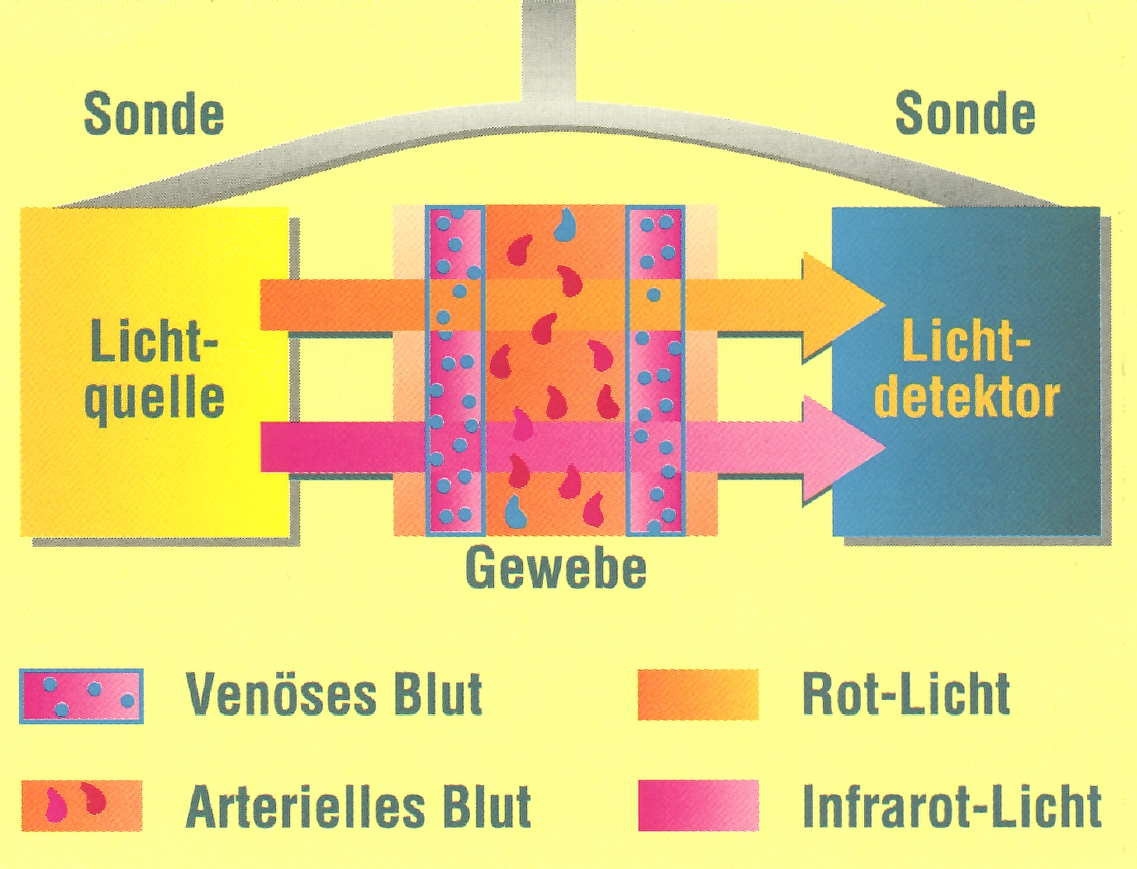
\includegraphics[scale=1.0]{images/pulsoxy.jpg}
	\caption{Veranschaulichung der Pulsoxymetrie\cite{messprinzip-pulsoxi}}
	\label{pic:pulsoxy}
\end{figure}

% Kurze Erklärung 
% reicht das oder noch mehr?
TODO:
bitte Korrektur lesen
Quelle einfügen
Quelle: Behandlungsassistenz „… in der Arztpraxis“ von Dr. Uta Groger, Cornelsen Verlag, 1. Auflage, 2007




\newpage
\section{Hauptteil} \label{sec:hauptteil}
\subsection{Hauptteil - Part1}
Text

%\bigskip
%\begin{figure}[H]
	%\visioToPDF{images/datei.pdf}
	%\centering
	%\includegraphics[scale=0.7]{images/datei.pdf}
	%\caption{Beschriftung}
	%\label{fig:layer}
%\end{figure}
%\bigskip

%\lstset{language=Java}
%\begin{lstlisting}[caption=Listing, label=lst:Listing]
%\end{lstlisting}

%\begin{shaded}
%Text in Textbox
%\end{shaded}

%\ref{sec:hauptteil}
%\cite{audio_architecture}



\newpage
\section{Fazit}
% muss rein (von Conrad):
% implementierte Anwendung und deren Funktionalitäten
% Verwendete Frameworks mit Begründung
% Beschreibung des Software-Designs
% Beschreibung des User Interfaces
% kurze Beschreibung der Bedienung der Anwendung
% weitere sinnvolle Angaben
% Verwendete Literatur und Quellen
\subsection{Retrospektive} \label{sec:Retrospektive}

% Retrospektive (kritischer Rückblick, Vergleich zu ursprüngliche Planung)
% - Schwierigkeit bei der Entscheidung, was schaffen wir in der vorgegen Zeit?
% - Übertragung von Smartphone zur GUI nicht über Bluetooth möglich 
% - Print Dialog
% Ausblick (Wie kann das Projekt weiter entwickelt werden)
\subsection{Ausblick} \label{sec:Ausblick}
Wie schon im Konzeptpapier erwähnt, besteht die Möglichkeit, das Projekt \textit{HeartRate2Go} zu publizieren und es so anderen Anwendern zugänglich zu machen. Hierzu könnte es durch weitere Funktionen erweitert werden. Einige dieser Anwendungen finden sich schon im Konzeptpapier unter 2.b. Optionale Funktionen, zum Beispiel: das Anlegen von Benutzerprofilen. \\ Dies geschieht derzeit nur ansatzweise, die gesendeten Werte werden für jedes Benutzerprofil des Betriebssystems separat abgespeichert. Jedoch ist eine Anamneseabfrage noch nicht möglich. In dieser würde nach Alter, Geschlecht, Größe, Gewicht, maximaler und minimaler Pulswert für die beiden Messwerttypen gefragt werden. So wäre auch eine erste Einschätzung der gemessenen Werte möglich.
\\
Ein anderer Punkt, ist die Berechnung des Kalorienverbrauchs. Zwar wird während einer Aktivitätsmessung die Anzahl der Schritte angezeigt, jedoch war es leider in der vorgegeben Zeit nicht möglich, der dadurch resultierende Kalorienverbrauch zu errechnen. Hierfür ist auch die Schrittlänge nötig, die mit einem Benutzerprofil einhergeht. \\
Des Weiteren stand zur Diskussion, ob dem Nutzer die Möglichkeit gegeben werden soll, Marker zusetzen, die eine besondere Situation kennzeichnen und in der späteren Ansicht speziell angezeigt werden. Dies ist bei einer, vom Hausarzt angeordneten, Langzeit-EKG-Messung ein wichtiger Teil, auch für die spätere Bewertung der Messung. \\
Da das \textit{HeartRate2Go-Programm} auf allen Betriebssysteme läuft, wäre eine App für das iOS-Betriebssystem auch praktisch. Der Zeit existiert die \textit{HeartRate2Go-App} nur für Android. Die Erstellung einer iOS-App war jedoch leider nicht möglich, da hierfür keine passende Apple-Komponenten zur Verfügung standen.\\
Die Umsetzung der genannten Punkte scheiterte an der begrenzten Zeit, die für dieses Projekt zur Verfügung stand. \\
% - Messung per Smartphone
% - siehe Konzeptpaper (fehlende Nice-to-have Lasten)
% 	- Benutzerprofile anlegen und abspeichern mit Anamneseabfrage
% 	- Berechnung des Kalorienverbrauchs
% - Marker setzten
% - iOS-App

% Drucken und mit abgeben:
% Ausgabe der Projektarbeit und Nutzungsvereinbarung
% Ehrenwörtliche Erklärung

\newpage

%% Literaturverzeichnis
%% ==> Eine Datei 'literatur.bib' wird hierf�r ben�tigt.
%% ==> Sie m�ssen hierf�r BibTeX verwenden (Projekt | Eigenschaften... | BibTeX)

\addcontentsline{toc}{section}{Literaturverzeichnis}
%\nocite{*} %Auch nicht-zitierte BibTeX-Eintr�ge werden angezeigt.
%\bibliographystyle{alpha} %Art der Ausgabe: plain / apalike / amsalpha / ...
%\bibliography{literatur} %Eine Datei 'literatur.bib' wird hierf�r ben�tigt.

\def\bibfont{\footnotesize}
\printbibliography[title={Literaturverzeichnis}]

%% Abbildungsverzeichnis
%\clearpage
%\addcontentsline{toc}{section}{Abbildungsverzeichnis}
%\listoffigures

%% Tabellenverzeichnis
%\clearpage
%\addcontentsline{toc}{section}{Tabellenverzeichnis}
%\listoftables


%%%%%%%%%%%%%%%%%%%%%%%%%%%%%%%%%%%%%%%%%%%%%%%%%%%%%%%%%%%%%
%% ANH�NGE
%%%%%%%%%%%%%%%%%%%%%%%%%%%%%%%%%%%%%%%%%%%%%%%%%%%%%%%%%%%%%
\appendix
%% ==> Schreiben Sie hier Ihren Text oder f�gen Sie externe Dateien ein.

%\input{Dateiname} %Eine Datei 'Dateiname.tex' wird hierf�r ben�tigt.

\end{document}

